%!TEX root = main.tex

\chapter{Trigonométrie}
\label{chapter:trigo}


\section{Introduction}

La trigonométrie est une branche des mathématiques qui étudie les relations entre les angles et les côtés des triangles. Bien que souvent perçue comme une discipline théorique, elle est en réalité un outil fondamental dans de nombreux domaines techniques, notamment en génie civil. Que ce soit pour concevoir des infrastructures, réaliser des levés topographiques ou calculer des pentes, la trigonométrie permet aux ingénieurs de résoudre des problèmes concrets avec précision et efficacité.

En guise d'exemple concret, imaginons un ingénieur  voulant mesurer la hauteur d'un bâtiment en utilisant un dispositif de mesure des angles par rapport à l'horizontale (théodolite). Voici comment la trigonométrie entre en jeu. L'ingénieur place le théodolite à une distance $d$ du bâtiment et mesure l'angle $\theta$ entre le sol et le sommet du bâtiment. En utilisant la fonction tangente, qui relie l'angle à la hauteur $h$ et à la distance $d$, la trigonométrie donne la relation $\tan(\theta) = \frac{h}{d}$. La hauteur $h$ du bâtiment peut alors être calculée comme $h = d \, \tan(\theta)$.

% ICI shéma d'illustration

Ce chapitre vise à vous fournir une compréhension des principaux concepts trigonométriques.  
Vous serez  familiarisé avec les fonctions trigonométriques essentielles, notamment le sinus, le cosinus et la tangente.
L'objectif principal est d'être capable d'appliquer les relations trigonométriques pour résoudre des problèmes concrets, comme le calcul de distances, de hauteurs ou de pentes.
En combinant théorie et pratique, ce chapitre vous préparera à utiliser la trigonométrie comme un outil puissant et polyvalent dans votre future carrière en génie civil.


\section{Un point sur les unités d'angle}


La mesure des angles est essentielle dans de nombreux domaines, notamment en mathématiques, en physique, en ingénierie et en topographie. Il existe plusieurs unités pour exprimer les angles, chacune ayant ses avantages et ses applications spécifiques. Nous allons explorer les trois principales unités : les \textbf{radians}, les \textbf{degrés} et les \textbf{grads} (ou \textbf{gons}), en mettant en lumière leur utilisation, en particulier en topographie.


\textbullet\ Le \textbf{radian} est l'unité\footnote{Pour être tout à fait exact, le radian n'est pas considérée comme une unité en physique car il définit u rapport de longueur. Ici, on s'autorisera cet abus de language.} de mesure d'angle dans le système international (SI). Un radian est défini comme l'angle sous-tendu par un arc de cercle dont la longueur est égale au rayon du cercle. Autrement dit, si un arc de longueur $R$ est tracé sur un cercle de même rayon, l'angle correspondant au centre du cercle est de 1 radian.
Un cercle complet correspond à un angle de $2\pi$ radians, car la circonférence d'un cercle est $2\pi R$. Ainsi,
$360^\circ$ représente $2\pi$~radians.
On voit alors que l'unité de radian pour un angle est naturel pour les calculs mathématiques, les radians simplifient les formules en analyse mathématique, notamment pour les dérivées et les intégrales des fonctions trigonométriques.


\textbullet\  Le \textbf{degré} est une unité de mesure d'angle largement répandue. Un degré est défini comme $\frac{1}{360}$ d'un cercle complet. Ainsi, un cercle complet mesure $360^\circ$.
%
Par exemple, en navigation ou cartographie, les degrés sont utilisés pour exprimer les latitudes et longitudes. De façon générale, les degrés sont souvent utilisés dans les cours de géométrie pour leur simplicité et leur \og familiarité \fg.
Pour convertir des degrés en radians, il suffit de multiplier par $\pi/180$.
Par exemple, $180^\circ = \pi$ radians.


\textbullet\   Le \textbf{grad} (ou \textbf{gon} du grec \textit{gônia} qui signifie angle) est une unité de mesure d'angle moins courante, mais très utile en topographie. Un gon est défini comme \( \frac{1}{400} \) d'un cercle complet. 
Les gons permettent des calculs plus précis pour les mesures angulaires sur le terrain.
Comme ils divisent le cercle en 400 unités, ils sont compatibles avec le système métrique décimal, ce qui peut faciliter les calculs et les conversions.

Pour convertir des gons en degrés ou en radians, on utilise les relations suivantes :
%
\begin{equation*}
1 \text{ gon} = 0.9^\circ = \frac{\pi}{200} \text{ radians}
\end{equation*}
%
Ainsi, un angle droit mesure  \num{100} grades ou $\frac{\pi}{2}$ radians.


\begin{bclogo}[arrondi=0.1,barre=snake,noborder=true,logo=\bclampe]{Astuce}
Pour utiliser correctement les fonctions trigonométriques sur une calculatrice de collège, 
il faut vérifier le mode d'angle sélectionné. Les calculatrices de collège proposent au moins deux modes~: les degrés (\textsc{Deg}) et les radians (\textsc{Rad}). Certaines calculatrices offrent aussi le mode des grades (\textsc{Grad}).
%
Une erreur de mode peut donner des résultats totalement faux~: par exemple, $\sin(30)$ affichera \texttt{0.5} en mode \textsc{Deg} (pour $30^\circ$), mais environ \texttt{-0.988} en mode \textsc{Rad} (pour $30$~radians). Pensez toujours à vérifier ce réglage avant de commencer vos calculs !
\end{bclogo}


\begin{exo}
Convertir : ...
\end{exo}

\begin{sol}
blabla
\end{sol}



\section{Les fonctions sinus, cosinus et tangente}



Les fonctions trigonométriques sont des outils fondamentaux en mathématiques, particulièrement en géométrie et en analyse. Elles permettent de décrire les relations entre les angles et les côtés des triangles, ainsi que de modéliser des phénomènes périodiques comme les ondes ou les mouvements circulaires.


\begin{bclogo}[arrondi=0.1,barre=snake,noborder=true,logo=\bcattention]{Parenthèses}
Parfois, on peut écrire une fonction trigonométrique sans mettre de parenthèses, à condition qu'il n'y ait pas de risque de confusion. Par exemple, il est courant d'écrire $\cos \theta$ plutôt que $\cos(\theta)$, car on comprend facilement que l'angle est $\theta$.
En revanche, on évite d'écrire $\cos \omega t$ à la place de $\cos(\omega t)$, car cela pourrait prêter à confusion : on pourrait croire qu'il s'agit de $\cos\omega$ multiplié par $t$.
\end{bclogo}

\begin{bclogo}[arrondi=0.1,barre=snake,noborder=true,logo=\bcattention]{Carré du cosinus}
Toujours dans l'idée d'éviter les confusions, on utilise une notation particulière pour écrire le carré (ou une autre puissance) d'une fonction trigonométrique. Par exemple, on écrit généralement $\cos^2(x)$ plutôt que $\cos(x)^2$.
Cette façon d'écrire est plus courte, mais elle veut dire exactement la même chose : $\cos^2(x)$ signifie le carré du cosinus de $x$, c'est-à-dire $(\cos(x))^2$.
Attention à ne pas confondre $\cos^2(x)$ avec $\cos(x^2)$ ! Dans le premier cas, on élève le résultat du cosinus au carré, alors que dans le second, on calcule le cosinus du carré de $x$. Ce n'est pas du tout la même chose.
\end{bclogo}

\textbullet\  \textbf{La fonction sinus} associe à un angle $\theta$ (exprimé dans l'unité de son choix) le rapport entre la longueur du côté opposé à cet angle et la longueur de l'hypoténuse dans un triangle rectangle. Mathématiquement, pour un angle $\theta$ dans un triangle rectangle, on a :
\begin{equation*}
\sin(\theta) = \frac{\text{côté opposé}}{\text{hypoténuse}}
\end{equation*}

La fonction sinus est  \textbf{périodique} de période $2\pi$, \textbf{impaire} (symétrique par rapport à l'origine), et définie pour tout réel $x \in \mathbb{R}$. Elle prend ses valeurs dans l'intervalle $[-1,\,1]$. 

\begin{center}
    \begin{tikzpicture}
        \begin{axis}[
            mathbook,
            width=\textwidth,
            height=6cm,
            xmin=-3*pi-1, xmax=3*pi+1,
            ymin=-1.2, ymax=1.2,
            xtick={-7.85, -4.71, -1.57, 0, 1.57, 4.71, 7.85},
            xticklabels={$-\frac{5\pi}{2}$, $-\frac{3\pi}{2}$, $-\frac{\pi}{2}$, $0$, $\frac{\pi}{2}$, $\frac{3\pi}{2}$, $\frac{5\pi}{2}$},
        ]
            \addplot[black,line width = 1.5pt,domain=-3*pi:3*pi]{sin(deg(x))};
        \end{axis}
    \end{tikzpicture}
\end{center}

Sa courbe, appelée \textit{sinusoïde}, oscille entre \num{-1} et \num{1} et passe par des \textit{maxima} en $x = \frac{\pi}{2} + 2k\pi$ (valeur \num{1}), des \textit{minima} en $x = \frac{3\pi}{2} + 2k\pi$ (valeur \num{-1}), et s'annule en $x = k\pi$ ($k \in \mathbb{Z}$). Elle est croissante sur $\left[-\frac{\pi}{2}, \frac{\pi}{2}\right]$ et décroissante sur $\left[\frac{\pi}{2}, \frac{3\pi}{2}\right]$, reflétant sa dérivée $\sin'(x) = \cos(x)$.


\textbullet\  \textbf{La fonction cosinus} associe à un angle $\theta$ le rapport entre la longueur du côté adjacent à cet angle et la longueur de l'hypoténuse dans un triangle rectangle. Mathématiquement, on écrit :
%
\begin{equation*}
\cos(\theta) = \frac{\text{côté adjacent}}{\text{hypoténuse}}
\end{equation*}
%
Comme la fonction sinus, la fonction cosinus est  \textbf{périodique} de période $2\pi$, \textbf{paire} (symétrique par rapport à l'axe des ordonnées), et définie pour tout réel $x$ de $\mathbb{R}$. Elle prend ses valeurs dans l'intervalle $[-1,\,1]$.

\begin{center}
    \begin{tikzpicture}
        \begin{axis}[
            mathbook,
            width=\textwidth,
            height=6cm,
            xmin=-3*pi-1, xmax=3*pi+1,
            ymin=-1.2, ymax=1.2,
            xtick={-9.42, -6.28, -3.14, 0, 3.14, 6.28, 9.42},
            xticklabels={$-3\pi$, $-2\pi$, $-\pi$, $0$, $\pi$, $2\pi$, $3\pi$},
        ]
            \addplot[black,line width = 1.5pt, domain=-3*pi:3*pi]{cos(deg(x))};
        \end{axis}
    \end{tikzpicture}
\end{center}

Sa courbe oscille entre -1 et 1 et passe par des \textit{maxima} en $x = 2k\pi$ (valeur \num{1}), des \textit{minima} en $x = \pi + 2k\pi$ (valeur \num{-1}), et s'annule en $x = \frac{\pi}{2} + k\pi$ ($k \in \mathbb{Z} $). Elle est décroissante sur $[0, \pi]$ et croissante sur $[\pi, 2\pi]$, reflétant sa dérivée $\cos'(x) = -\sin(x)$.


\textbullet\  \textbf{La fonction tangente} est définie comme le rapport entre le sinus  et le cosinus :
\begin{equation*}
\tan(\theta) = \frac{\sin(\theta)}{\cos(\theta)}
\end{equation*}
%
Elle représente également le rapport entre le côté opposé et le côté adjacent dans un triangle rectangle :
\begin{equation*}
\tan(\theta) = \frac{\text{côté opposé}}{\text{côté adjacent}}
\end{equation*}
%
Contrairement aux fonctions sinus et cosinus, la fonction tangente n'est pas bornée et présente des asymptotes verticales aux angles $x$ où $\cos(x) = 0$, donc pour $x = \frac{\pi}{2} + k\pi \quad \forall k \in \mathbb{Z}$.


\begin{center}
    \begin{tikzpicture}
        \begin{axis}[
            mathbook,
            width=\textwidth,
            height=6cm,
            xmin=-3*pi-1, xmax=3*pi+1,
            ymin=-4, ymax=4,
            xtick={-9.42, -6.28, -3.14, 0, 3.14, 6.28, 9.42},
            xticklabels={$-3\pi$, $-2\pi$, $-\pi$, $0$, $\pi$, $2\pi$, $3\pi$},
            tick label style={inner sep=1pt, font=\scriptsize},
            xticklabel style={yshift=-8pt},
            restrict y to domain=-4:4, % Limite l'affichage de la tangente
        ]
            \addplot[black,line width = 1.5pt,domain=-3*pi:3*pi,samples=5000]{tan(deg(x))};
            
        \end{axis}
    \end{tikzpicture}
\end{center}

La fonction est \textbf{périodique} de période $\pi$, \textbf{impaire} (symétrique par rapport à l'origine), et définie pour tout réel $x \neq \frac{\pi}{2} + k\pi$ ($k \in \mathbb{Z}$). Sa courbe présente des \textbf{asymptotes verticales} aux points $x = \frac{\pi}{2} + k\pi$ et oscille entre $-\infty$ et $+\infty$. Elle s'annule en $x = k\pi$ ($k \in \mathbb{Z}$) et est croissante sur chaque intervalle de son domaine de définition. Sa dérivée est donnée par $\tan'(x) = 1 + \tan^2(x)$.


% conseil
\begin{bclogo}[arrondi=0.1,barre=snake,noborder=true,logo=\bclampe]{Astuce}
Plutôt que de s'appuyer systématiquement sur le moyen mnémotechnique \og SOH~CAH~TOA \fg, il est préférable de travailler à mémoriser et comprendre les relations fondamentales dans un triangle rectangle.
Avec de la pratique, ces relations deviennent naturelles et leur utilisation intuitive et rapide. De façon générale, les astuces apprises avant le bac peuvent être très utiles pour débuter, mais l'objectif est de s'en détacher progressivement pour gagner en aisance et en profondeur mathématique, même si l'objectif n'est pas de devenir un grand mathématicien.
\end{bclogo}

\begin{exo}
Exercices dans des triangles rectangles
\end{exo}

\begin{sol}
Correction des exercices dans des triangles rectangles
\end{sol}

\begin{exo}

\begin{enumerate}
\item La fonction $x(t) = A \cos(\omega t + \phi)$ est-elle paire, impaire, ou ni l'une ni l'autre ? Justifier.

% pour formule d'addition
%\item Montrer que $\cos(\omega t + \phi)$ peut s'écrire comme une combinaison linéaire de $\sin(\omega t)$ et  $\cos(\omega t)$.

\item Quelle est la période $T$ de $x(t) = 3 \cos(4t + \pi/3)$ ?

\item La fonction $z(t) = \cos(t)+\sin(2t)$ est-elle périodique ? Si oui, quelle est sa période ? Calculer $z(\tfrac{\pi}{2})$ et $z(\pi)$.

\item Quelle est la période de $\tan(\omega t)$ ? La fonction est-elle paire, impaire, ou ni l'une ni l'autre ? Justifier.
\end{enumerate}

\end{exo}

\begin{sol}

\begin{enumerate}
\item La fonction $x(t) = A \cos(\omega t + \phi)$ n'est ni paire ni impaire en général, sauf dans des cas particuliers. Pour le montrer de façon purement graphique [...]

\item On veut trouver la plus petite durée $T > 0$ telle que $x(t+T) = x(t)\ \forall t$. En particulier, pour $t=0$, $x(T) = x(0)$ et donc :
\begin{equation*}
\cos(4T + \tfrac{\pi}{3}) = \cos(\tfrac{\pi}{3} + 2k\pi) \implies 4T = 2k\pi  \implies T = \frac{k\pi}{2}
\end{equation*}
La plus petite valeur strictement positive est $T=\tfrac{\pi}{2}$ en prenant $k=1$.
On retiendra que, de façon générale, la période de $\cos(\omega t + \phi)$ ou de $\sin(\omega t + \phi)$ est $T = \frac{2 \pi}{\omega}$. 

\item On sait que la période de $\cos(t)$ est  $T_1= 2 \pi$, et que la période de $\sin(2t)$ est $T_2=\frac{2\pi}{2} = \pi$. La période $T_1$ est un multiples de $T_2$, $T_1 = 2 T_2$. Ce rapport d'exactement 2, un nombre entier, rend la fonction $z(t)$ également périodique, de période $2\pi$ (plus petit multiple commun à $T_1$ et $T_2$).

$z(\tfrac{\pi}{2}) = \cos(\tfrac{\pi}{2}) + \sin(2 \tfrac{\pi}{2}) = 0 + \sin(\pi) = 0$

$z(\pi) = \cos(\pi) + \sin(2 \pi) = (-1) + 0 = -1$

\item On sait que la fonction tangente est périodique de période $\pi$, donc $\tan(x+\pi) = \tan(x)$. Par conséquent, en remplaçant $x$ par $\omega t$, on obtient $\tan(\omega t+\pi) = \tan(\omega t)$. Cherchons, $T>0$ tel que $\tan(\omega (t+T)) = \tan(\omega t+\omega T) = \tan(\omega t)$. On identifie alors que $\omega T = \pi$, donc $T=\frac{\pi}{\omega}$.

La fonction $\tan(\omega t)$ est impaire comme l'est la fonction tangente. 
\end{enumerate}


\end{sol}


\section{Le cercle trigonométrique} % est un très bon ami !


Le cercle trigonométrique est un outil fondamental pour relier les notions d'angles et de fonctions trigonométriques. 
Il constitue un point de passage essentiel entre la géométrie et l'analyse, et joue un rôle clé dans de nombreuses applications comme  la mesure d'angles, le calcul de pentes, la topographie, et la modélisation de phénomènes périodiques (oscillatoires).


On appelle \textbf{cercle trigonométrique} le cercle centré à l'origine d'un repère orthonormé et de rayon unitaire. 
Le sens positif de rotation est le sens \textbf{anti-horaire}.  
Chaque point $M$ de ce cercle correspond à un angle orienté $\theta$ dont  les coordonnées  sont directement liées aux valeurs du cosinus et du sinus comme illustré ci-après.

\begin{center}
\begin{tikzpicture}

\cercletrigo{2cm}{0.9cm}
\draw[line width=1pt, black, line cap=round] (0,0) -- (53:2);
\draw[>=angle 60, ->, line width=1pt, line cap=round] (0:0.8) arc (0:53:0.8);
\draw ({53/2}:1) node[]{$\theta$};
\draw ({cos(53)*2},0) node[below]{$\cos \theta$};
\draw (0,{sin(53)*2}) node[left]{$\sin \theta$};

\draw (3,0) node[right]{\og cosinus \fg};
\draw (0,3) node[above]{\og sinus \fg};

\draw (-2,0) node[fill=white, left]{-1};
\draw (2,0) node[fill=white, right]{1};
\draw (0,-2) node[fill=white, below]{-1};
\draw (0,2) node[fill=white, above]{1};

\draw[line width=1pt, black, line cap=round, dotted] ({cos(53)*2},{sin(53)*2}) -- ({cos(53)*2},0);
\draw[line width=1pt, black, line cap=round, dotted] ({cos(53)*2},{sin(53)*2}) -- (0,{sin(53)*2});

\draw[>=angle 60, ->, line width=1pt, line cap=round] (20:2.8) arc (20:60:2.8);
\draw[>=angle 60, ->, line width=1pt, line cap=round] (-20:2.8) arc (-20:-60:2.8);
\draw (40:3.2) node[]{\textcircled{+}};
\draw (-40:3.2) node[]{\textcircled{-}};

\end{tikzpicture}
\end{center}

% il faut commenter le cercle

Le cercle trigonométrique doit être considéré comme un \og très bon ami \fg\ parce qu'il permet de visualiser intuitivement les relations entre les fonctions trigonométriques et les angles.  
Grâce à lui, on comprend d'un simple coup d'œil pourquoi $\sin^2\theta + \cos^2\theta = 1$, 
ou encore comment les signes de $\sin\theta$ et $\cos\theta$ varient selon le quadrant considéré.  
Dans de nombreuses situations, revenir au cercle trigonométrique 
permet de vérifier rapidement la cohérence d'un calcul ou d'une mesure angulaire.


\section{Angles remarquables}

Les angles remarquables sont des angles pour lesquels les valeurs des fonctions trigonométriques $\sin$, $\cos$ et $\tan$ peuvent être déterminées exactement, souvent à l'aide de triangles particuliers ou de propriétés géométriques. Voici les angles les plus courants et leurs valeurs associées :


Ces angles ($0^\circ$, $30^\circ$, $45^\circ$, $60^\circ$ et $90^\circ$) sont souvent étudiés dans le contexte d'un triangle rectangle ou d'un cercle trigonométrique. Leurs valeurs trigonométriques peuvent être déterminées à l'aide des triangles suivants :

% AJOUTER ????


\begin{center}
\begin{tabular}{ccccc}
\toprule
\multicolumn{2}{c}{Angle $\theta$}  & & & \\
\cmidrule{1-2}
(degré) & (radian) & $\sin\theta$ & $\cos\theta$ & $\tan\theta$ \\
\midrule
$0^\circ$ & 0 & 0 & 1 & 0 \\[2mm]
$30^\circ$ & $\dfrac{\pi}{6}$ & $\dfrac{1}{2}$ & $\dfrac{\sqrt{3}}{2}$ & $\dfrac{1}{\sqrt{3}}$ \\[2mm]
$45^\circ$ & $\dfrac{\pi}{4}$ & $\dfrac{\sqrt{2}}{2}$ & $\dfrac{\sqrt{2}}{2}$ & 1 \\[2mm]
$60^\circ$ & $\dfrac{\pi}{3}$ & $\dfrac{\sqrt{3}}{2}$ & $\dfrac{1}{2}$ & $\sqrt{3}$ \\[2mm]
$90^\circ$ & $\dfrac{\pi}{2}$ & 1 & 0 & -- \\[2mm]
\bottomrule
\end{tabular}
\end{center}


Ces valeurs sont souvent mémorisées pour faciliter les calculs et sont essentielles pour comprendre les propriétés des fonctions trigonométriques.
Ces angles remarquables peuvent être utiles pour simplifier les calculs trigonométriques, résoudre des équations trigonométriques, ou encore déterminer des valeurs exactes dans des problèmes géométriques ou physiques.


% astuces ne pas retenir bêtement, mais remarquer qu'il n'y a que peu de valeurs

\begin{center}
\begin{tikzpicture}

\cercletrigo{1.5cm}{0.4cm}
\draw[line width=1pt, black, line cap=round] (0,0) -- (45:1.5);
%\draw[line width=1pt, black, line cap=round] (0,1.5) -- (45:1.5);
\draw (45:1.8) node[]{$\tfrac{\pi}{4}$};
\draw[line width=1pt, black, line cap=round,dotted] (0,{sin(45)*1.5}) -- (45:1.5);
\draw[line width=1pt, black, line cap=round,dotted] ({cos(45)*1.5},0) -- (45:1.5);
\draw ({cos(45)*1.5},0)  node[below]{$\tfrac{1}{\sqrt{2}}$};
\draw (0,{sin(45)*1.5})  node[left]{$\tfrac{1}{\sqrt{2}}$};

\begin{scope}[xshift=4.5cm]
\cercletrigo{1.5cm}{0.4cm}
\draw[line width=1pt, black, line cap=round] (0,0) -- (30:1.5);
\draw[line width=0.5pt, black, line cap=round] (0,1.5) -- (30:1.5);
\draw (30:1.8) node[]{$\tfrac{\pi}{6}$};
\draw[line width=1pt, black, line cap=round,dotted] (0,{sin(30)*1.5}) -- (30:1.5);
\draw[line width=1pt, black, line cap=round,dotted] ({cos(30)*1.5},0) -- (30:1.5);
\draw ({cos(30)*1.5 - 0.1},0)  node[below]{$\tfrac{\sqrt{3}}{2}$};
\draw (0,{sin(30)*1.5})  node[left]{$\tfrac{1}{2}$};
\end{scope}

\begin{scope}[xshift=9cm]
\cercletrigo{1.5cm}{0.4cm}
\draw[line width=1pt, black, line cap=round] (0,0) -- (60:1.5);
\draw[line width=0.5pt, black, line cap=round] (1.5,0) -- (60:1.5);
\draw (60:1.8) node[]{$\tfrac{\pi}{3}$};
\draw[line width=1pt, black, line cap=round,dotted] (0,{sin(60)*1.5}) -- (60:1.5);
\draw[line width=1pt, black, line cap=round,dotted] ({cos(60)*1.5},0) -- (60:1.5);
\draw ({cos(60)*1.5},0)  node[below]{$\tfrac{1}{2}$};
\draw (0,{sin(60)*1.5-0.2})  node[left]{$\tfrac{\sqrt{3}}{2}$};
\end{scope}

\end{tikzpicture}
\end{center}

%\subsection{Autres angles remarquables}

D'autres angles, comme $18^\circ\,(\frac{\pi}{10})$, $36^\circ\,(\frac{\pi}{5})$, $54^\circ\,(\frac{3\pi}{10})$ et $72^\circ\,(\frac{2\pi}{5})$, sont également remarquables et peuvent être étudiés à l'aide de triangles d'or ou de pentagones réguliers. Par exemple :
%
\begin{itemize}
    \item[\ding{42}] $\sin(18^\circ) = \frac{\sqrt{5} - 1}{4}, \quad \cos(18^\circ) = \frac{\sqrt{10 + 2\sqrt{5}}}{4}$
    \item[\ding{42}] $\sin(36^\circ) = \frac{\sqrt{10 - 2\sqrt{5}}}{4}, \quad \cos(36^\circ) = \frac{\sqrt{5} + 1}{4} $
\end{itemize}
%
Bien entendu, il n'est absolument pas nécessaire de mémoriser toutes ces formules, et nous verrons plus loin comment ils peuvent être établis.

%\subsection{Utilisation des angles remarquables}

\begin{exo}
\noindent \ding{45} Donner la valeur exacte des expressions suivantes :

\begin{tasks}(3)
\task $\sin(30^\circ)$
\task $ \cos(\tfrac{\pi}{3})$
\task $\sin(30^\circ) + \cos(60^\circ)$
\task $\dfrac{\sin(60^\circ)}{\cos(30^\circ)}$
\task $\cos(\pi + \tfrac{\pi}{3})$
\task $\cos^2(30^\circ) + \sin^2(30^\circ)$
\end{tasks}

\end{exo}

\begin{sol}

\begin{tasks}(2)
\task $\sin(30^\circ) = \dfrac{\sqrt{3}}{2}$
\task $ \cos(\tfrac{\pi}{3}) = \dfrac{1}{2}$
\task $\sin(30^\circ) + \cos(60^\circ) = \dfrac{1}{2}+\dfrac{1}{2}= 1$
\task $\dfrac{\sin(60^\circ)}{\cos(30^\circ)}$
\task $\cos(\pi + \tfrac{\pi}{3})$
\task $\cos^2(30^\circ) + \sin^2(30^\circ)$
\end{tasks}

\end{sol}


\section{Angles associés}

En trigonométrie, les angles associés permettent de relier les valeurs des fonctions trigonométriques pour différents angles en utilisant des propriétés géométriques et algébriques. Ces relations sont particulièrement utiles pour simplifier des expressions ou résoudre des équations trigonométriques.
%
Par exemple, en utilisant la relation de complémentarité, l'expression $\sin(\tfrac{\pi}{2} - x) + \cos(x)$ peut se simplifier en $ \cos(x) + \cos(x) = 2\cos(x)$.

%\subsection{Relations fondamentales entre angles associés}

Les angles associés sont souvent obtenus par des transformations géométriques comme la complémentarité, la supplémentarité, l'opposition, la périodicité ou la symétrie (cette dernière notion étant liée à la parité). Voici quelques relations parmi les plus importantes :

\begin{center}
\begin{tabular}{ccc}
\toprule
 sinus  & cosinus & tangent \\
\midrule
 $\sin(\tfrac{\pi}{2}-a) = \cos(a)$ & $\cos(\tfrac{\pi}{2}-a)=\sin(a)$ & $\tan(\tfrac{\pi}{2}-a) = \cot(a)$ \\
 $\sin(\pi - a) = \sin(a)$ & $\cos(\pi - a) = -\cos(a)$ & $\tan(\pi - a) = -\tan(a)$ \\
 $\sin(\pi + a) = -\sin(a)$ & $\cos(\pi + a) = -\cos(a)$ & $\tan(\pi + a) = \tan(a)$ \\
 $\sin(a + 2\pi) = \sin(a)$ & $\cos(a + 2\pi) = \cos(a)$ & $\tan(a + \pi) = \tan(a)$ \\
 $\sin(-a) = -\sin(a)$ & $\cos(-a) = \cos(a)$ & $\tan(-a) = -\tan(a)$ \\
\bottomrule
\end{tabular}
\end{center}


\begin{bclogo}[arrondi=0.1,barre=snake,noborder=true,logo=\bcattention]{Cotangente}
La fonction cotangente, notée $\cot(x)$, correspond à l'inverse de la tangente : $\cot(x) = \tfrac{1}{\tan(x)}$. Il ne faut pas la confondre avec $\tan^{-1}(x)$, qui ne désigne pas une puissance inverse mais la fonction réciproque de la tangente, appelée aussi $\arctan(x)$. Autrement dit, $\cot(x)$ représente l'inverse de la tangente de $x$, tandis que $\tan^{-1}(x)$ (ou $\arctan(x)$) désigne l'angle dont la tangente vaut $x$. La fonction $\arctan$ sera étudiée plus loin.
\end{bclogo}

Dans le tableau précédent, les transformations sont données dans l'ordre suivant : complémentarité,  supplémentarité, opposition, périodicité et symétrie.
Ces termes sont bien sûr utiles, mais plutôt que de s'enfermer dans des définitions, explorons comment le cercle trigonométrique peut révéler, d'un seul regard, toutes ces correspondances.



%\subsection{Visualisation sur le cercle unité}

Les relations des angles associés peuvent être visualisées sur le cercle unité. Par exemple, l'angle \(\frac{\pi}{2} - a\) est le reflet de l'angle \(a\) par rapport à l'axe vertical du cercle unité, ce qui explique pourquoi \(\cos\left(\frac{\pi}{2} - a\right) = \sin(a)\).
[...]

\begin{comment}
\subsection{Cas particuliers}

- **Angles négatifs** : Grâce à la symétrie, on peut exprimer les fonctions trigonométriques d'angles négatifs en termes d'angles positifs.
- **Angles supérieurs à \(2\pi\)** : La périodicité des fonctions trigonométriques permet de ramener l'étude de ces angles à celle d'angles dans l'intervalle \([0, 2\pi]\).
\end{comment}

\begin{exo}
\noindent Simplifier les expressions suivantes

\begin{tasks}(2)
\task $\dfrac{\sin(\frac{\pi}{2} - \theta)}{\cos(\pi+\theta)}$
\task $\dfrac{\sin(\pi- x)}{\cos(\pi+x)}$
\task $\dfrac{\sin(\frac{3\pi}{2} + x) \cos(\frac{\pi}{2})}{\tan(\pi- x) \sin(-x)}$
\task $\sin(\tfrac{5\pi}{2} - x) \cos(-x)$
\end{tasks}

\end{exo}


\begin{sol}

\begin{tasks}(2)
\task $\dfrac{\sin(\frac{\pi}{2} - \theta)}{\cos(\pi+\theta)} = -1$
\task $\dfrac{\sin(\pi- x)}{\cos(\pi+x)}  = -\tan(x)$
\task $\dfrac{\sin(\frac{3\pi}{2} + x) \cos(\frac{\pi}{2})}{\tan(\pi- x) \sin(-x)} = \dfrac{-\cos^2 (x)}{\sin(x)}$
\task $\sin(\tfrac{5\pi}{2} - x) \cos(-x) = \cos^2(x)$
\end{tasks}

\end{sol}




\section{Relations dans un triangle quelconque}


\subsection{Relation des sinus}

% dessin

\begin{equation*}
\dfrac{\sin (\alpha)}{a} = \dfrac{\sin (\beta)}{b} = \dfrac{\sin (\gamma)}{c} = \dfrac{2S}{abc}  
\end{equation*}


\subsection{Théorème d'Al Kashi}

% dessin

\begin{equation*}
\begin{cases}
 c^2 &= a^2 + b^2 - 2 a b \cos (\gamma) \\
 a^2 &= b^2 + c^2 - 2 b c \cos (\alpha) \\
 b^2 &= c^2 + d^2 - 2 c d \cos (\beta) 
\end{cases}  
\end{equation*}


\section{Principales formules trigonométriques}

\subsection{Pythagore dans le cercle trigonométrique}



\begin{equation*}
\cos^2(x) + \sin^2(x) = 1
\end{equation*}



\subsection{Formules d'addition}

\begin{equation*}
\vv{OA} \cdot \vv{OB} = \cos (b-a) = ...
\end{equation*}



\subsection{Formules de duplication}

À partir de formule d'addition
%
\begin{equation*}
\cos(2x) = \cos(x+x) = \cos(x)\cos(x) - \sin(x)\sin(x) 
\end{equation*}
%
d'où
%
\begin{equation*}
\boxed{\cos(2x)= \cos^2(x) - \sin^2(x)}
\end{equation*}
%
En introduisant le fait que $\cos^2(x) + \sin^2(x)=1$ on peut obtenir deux autres expressions :
\begin{equation*}
\cos(2x)= \cos^2(x) - \sin^2(x) + 1 - 1 = \cos^2(x) - \sin^2(x) + \left( \cos^2(x) + \sin^2(x) \right) - 1 
\end{equation*}
%
Ce qui conduit à :
%
\begin{equation*}
\boxed{
\cos(2x)=  2\cos^2(x)   - 1 
\quad\text{ou}\quad
\cos(2x)=  1 +  2\sin^2(x)
}
\end{equation*}


Blabla sin(2x) à partir de formule d'addition
%
\begin{equation*}
\sin(2x) = \sin(x+x) = \sin(x)\cos(x) + \sin(x)\cos(x) 
\end{equation*}
%
d'où
%
\begin{equation*}
\sin(2x)= 2\sin(x)\cos(x)
\end{equation*}

Ces formules sont très utiles pour simplifier des expressions.


% ICI tableau qui resume les formules



\begin{center} 
\begin{tabular}{l} 
\toprule 
Addition \\ 
\midrule 
$\sin(a+b) = \sin(a)\cos(b) + \cos(a)\sin(b)$ \\ [2mm] 
$\cos(a+b) = \cos(a)\cos(b) - \sin(a)\sin(b)$ \\[2mm]
\midrule 
Soustraction \\ 
\midrule 
$\sin(a-b) = \sin(a)\cos(b) - \cos(a)\sin(b)$ \\[2mm]  
$\cos(a-b) = \cos(a)\cos(b) + \sin(a)\sin(b)$ \\[2mm]
 \midrule 
 Duplication \\ 
 \midrule 
 $\sin(2a) = 2\sin(a)\cos(a)$ \\ [2mm] 
 $\cos(2a) = \begin{cases}
 \cos^2(a) - \sin^2(a) \\
  2\cos^2(a) - 1 \\
   1 - 2\sin^2(a)
   \end{cases}$ \\[2mm] 
 \midrule 
 Réduction \\ 
 \midrule 
 $\sin(\tfrac{a}{2}) = 
\langle \sin(\tfrac{a}{2})\rangle ^\pm \, 
 \sqrt{\dfrac{1 - \cos(a)}{2}}$ \\ [2mm]
 $\cos\!\left(\tfrac{a}{2}\right) = 
 \langle \sin(\tfrac{a}{2})\rangle ^\pm \,
 \sqrt{\dfrac{1 + \cos(a)}{2}}$ \\ 
 \bottomrule 
 \end{tabular} 
 \end{center}




\begin{exo}
\noindent  En utilisant les différentes formules trigonométriques :
%
\begin{itemize}
\item[\ding{42}]  Soit un angle $x$ tel que 
$\tan(x) = \frac{\sin(x)}{\cos(x)} = \frac{3}{4}$. 
Calculer la valeur de $\sin^2(x) - \cos^2(x)$.

\item[\ding{42}]  Sachant que $\sin(x) = \tfrac{2}{3}$, calculer la valeur de exacte de $\cos^2(x)$ sans utiliser de calculatrice.

\item[\ding{42}]  En utilisant la formule de duplication, simplifie l'expression suivante : $\cos(2x)$:
$\cos^2(3x) -  \sin^2(3x)$

\item[\ding{42}]  À partir de la valeur exacte du sinus et du cosinus de l'angle $\tfrac{\pi}{6}$, et en utilisant les formules de duplication, calculer les
valeurs exactes de $\cos(\tfrac{\pi}{12})$ et $\sin(\tfrac{\pi}{12})$.

\item[\ding{42}]  Calculer la valeur exacte de $\sin(2x)$ si $\sin(x) = \frac{3}{5}$ et $\cos(x) = \frac{4}{5}$ 
\end{itemize}
\end{exo}

\begin{sol}

TODO


\end{sol}



\section{Équations trigonométriques : cas des égalités de sinus, cosinus et tangente}



Pour résoudre l'équation $\cos(a) = \cos(b)$, les solutions générales sont données par :
\begin{equation*}
\begin{cases}
a &= b + 2k\pi \\ 
\text{ou}& \\
a &= -b + 2k\pi 
\end{cases}
\qquad \forall k \in \mathbb{Z}
\end{equation*}


Pour résoudre l'équation $\sin(a) = \sin(b)$, les solutions générales sont données par :
\begin{equation*}
\begin{cases}
a &= b + 2k\pi \\ 
\text{ou}& \\
a &= (\pi - b) + 2k\pi 
\end{cases}
\qquad  \forall k \in \mathbb{Z}
\end{equation*}


\begin{exo}
\end{exo}

\begin{sol}
\end{sol}


\section{Inégalités trigonométriques}

% méthode graphique basée sur le cercle trigo




\section{Fonctions trigonométriques réciproques}






